\appendix


\section{Experimental Settings}
\label{setup}

\paragraph{Model architecture}
The core architectures of our experimental model are detailed in Table~\ref{table:Architectures}. 
The model is configured with 20 layers and a hidden dimension size of 2048. Except for the first layer, all FFNs layers are replaced with MoE layers. We adopt the GQA attention mechanism~\citep{gqa} and integrate Rotary Position Embedding (RoPE)~\citep{rope}, enabling the model to support sequence lengths up to 8K tokens. For parameter initialization, all learnable parameters are randomly initialized using a standard deviation of 0.006. 
Under this configuration, the model consists of a total of 16.3 billion parameters, of which approximately 1.43 billion are activated for each token during inference.

\begin{table}[h]
  \small
  \caption{{\textbf{Detailed model architectures.}}}
  \label{table:Architectures}
  \centering
  \setlength{\tabcolsep}{5pt} %
  \begin{tabular}{cccccccccccc}
    \toprule
      & $n_{layers}$ & $d_{model}$ & $d_{ffn}$ & $d_{expert}$ &$n_{heads}$ & $n_{kv\_head}$ & $E$ & $E_a$ & $E_s$ & $N$ & $N_a$ \\
    \midrule
      & 20 & 2048 & 5120 & 512 & 16 & 4 & 256 & 8 & 1 & 16.3B & 1.43B \\
    \bottomrule
  \end{tabular}
\end{table}

\paragraph{Training hyperparameters}
We use the AdamW optimizer~\citep{adamw} with hyperparameters set as follows: $\beta_1 = 0.9$, $\beta_2 = 0.95$, and weight decay of 0.1. Gradient clipping~\citep{clipping} norm is set to 1.0. According to the scaling laws for MoE optimal hyper-parameters, the maximum learning rates were set to $3.74e{-4}$. The batch size is set to 2048, and with a maximum sequence length of 8K, each training batch contains 16M tokens.

\paragraph{Pre-training dataset}
The training data is sourced from a large-scale multilingual corpus created by the Ling Team, primarily covering English and Chinese, while also including various other languages. This corpus encompasses web text, mathematical materials, programming scripts, published literature, and diverse textual content. To validate model performance, we extracted a 10T-token subset from this corpus for training.




\paragraph{Evaluation setup}
\label{}
To evaluate performance, we consider a diverse suite of downstream tasks designed to provide a holistic assessment of model capabilities. For base model, tasks are grouped into several categories, such as: (a) General Knowledge/Reasoning (e.g., ARC~\citep{arc}, AGIEval~\citep{agieval}, OpenBookQA~\citep{openbookqa}, BBH~\citep{bbh}, WorldSense~\citep{worldsense}, PIQA~\citep{piqa}, hellaswag~\citep{hellaswag} and KOR-Bench~\citep{korbench}) (b) Language Understanding (e.g., race~\citep{race}, SQuAD 2.0~\citep{squad2}, TriviaQA~\citep{trivalqa}, NQ~\citep{nq} and winogrande~\citep{winogrande}) (c) Professional Knowledge (e.g., MMLU~\citep{mmlu}, CMMLU~\citep{cmmlu}, C-Eval~\citep{ceval}, MMLU-Pro~\citep{mmlu-pro}, GPQA~\citep{gpqa} and SuperGPQA~\citep{supergpqa}) (d) Math (e.g., GSM8K~\citep{gsm8k}, MATH~\citep{math}, gaokao~\citep{gaokao}, GSM-Plus~\citep{gsm-plus}, mgsm-zh~\citep{mgsm}, CMATH~\citep{cmath}, MathBench~\citep{mathbench}, minerva\_math~\citep{math}, college\_math~\citep{college-math} and cn\_middle\_school\_24) (e) Code (e.g., HumanEval~\citep{humaneval}, LiveCodeBench~\citep{livecodebench}, MBPP~\citep{mbpp}, HumanEval\_plus~\citep{mbpp+}, MBPP\_plus~\citep{mbpp+}, HumanEval\_cn~\citep{humaneval_cn}, HumanEval\_fim~\citep{fim} and CruxEval~\citep{cruxeval}). For SFT model, the categories and tasks are shown in Table \ref{inst_dataset_1} and \ref{inst_dataset_2}.    









\section{Details of Theoretical Connection Between Decay and Merging}
\label{app:Theoretical}
The core idea of checkpoint merging in this work is to take an ordered list of checkpoints, $[\theta_n, \theta_{n+1}, \dots, \theta_{n+k}]$, and apply a merge function to generate a single model $\hat{\theta}_{n+k}$. Here, $\theta_i \in \mathbb{R}^d$ represents the model's parameter vector at the $i$-th training iteration.

The most general form is a weighted average of the checkpoints:
\begin{equation}
    \hat{\theta}_{n+k} = \sum_{j=0}^{k} c_j \theta_{n+j}
    \label{eq:weighted_avg_appendix}
\end{equation}
where $\{c_j\}$ are non-negative weights that sum to one, i.e., $\sum_{j=0}^{k} c_j = 1$.

While intuitive, this formulation obscures a deeper connection to the training dynamics. We can reveal this link by expressing each checkpoint in terms of an initial checkpoint $\theta_n$ and the subsequent gradient updates.

We assume that the updates between checkpoints at different time steps are independent. Let $g_{i}$ be the gradient update vector (including the learning rate) at step $i$, such that the model is updated via $\theta_{i+1} = \theta_i - g_i$. Any checkpoint $\theta_{n+j}$ can therefore be written as the sum of an initial state $\theta_n$ and the sequence of negative gradient updates that followed:
\begin{equation}
    \theta_{n+j} = \theta_{n} - \sum_{l=1}^{j} g_{n+l-1}
    \label{eq:theta_as_gradient_sum_appendix}
\end{equation}

Substituting Eq. \ref{eq:theta_as_gradient_sum_appendix} into the general merging formula (Eq. \ref{eq:weighted_avg_appendix}) yields:
\begin{align}
    \hat{\theta}_{n+k} &= \sum_{j=0}^{k} c_j \left( \theta_n - \sum_{l=1}^{j} g_{n+l-1} \right) \\
    &= \left( \sum_{j=0}^{k} c_j \right) \theta_n - \sum_{j=0}^{k} c_j \sum_{l=1}^{j} g_{n+l-1} \\
    &= \theta_n - \sum_{j=1}^{k} c_j \sum_{l=1}^{j} g_{n+l-1} \label{eq:rearrange_sum_step1_app}
\end{align}

The double summation in Eq. \ref{eq:rearrange_sum_step1_app} can be rearranged by changing the order of summation. A gradient update $g_{n+i-1}$ is included in the sum for all checkpoints $\theta_{n+j}$ where $j \ge i$.
\begin{align}
    \sum_{j=1}^{k} c_j \sum_{l=1}^{j} g_{n+l-1} &= \sum_{i=1}^{k} \left( \sum_{j=i}^{k} c_j \right) g_{n+i-1}
\end{align}
This shows that a weight coefficient of $\sum_{j=i}^{k} c_j$ is applied to the gradient update $g_{n+i-1}$ from step $n+i-1$.
By defining a new set of weights for the gradient updates, $w_i = \sum_{j=i}^{k} c_j$, we arrive at the final equivalent expression for checkpoint merging:
\begin{equation}
    \hat{\theta}_{n+k} = \theta_n - \sum_{i=1}^{k} w_i \cdot g_{n+i-1}
    \label{eq:merge_as_gradient_reweighting_app}
\end{equation}
This equation demonstrates that merging checkpoints with weights $\{c_j\}$ is equivalent to applying a synthetic decay schedule defined by weights $\{w_i\}$ to the gradients accumulated after the base checkpoint $\theta_n$, and there exists a mapping between the merging weights ${c_j}$ and the effective learning rates ${w_i}$
\subsection{Proof of Theorem \ref{thm:inverse}}

We seek to find the unique checkpoint weights $\{c_j\}$ corresponding to a given desired sequence of gradient decay coefficients $\{w_i\}_{i=1}^k$. The relationship derived in the previous section is the starting point:
\begin{equation}
w_i = \sum_{j=i}^{k} c_j
\label{eq:w_from_c_proof}
\end{equation}

We can solve for the checkpoint weights $\{c_j\}$ by starting from the last element and working backwards.

For $i = k$, the sum in Eq. \ref{eq:w_from_c_proof} has only one term:
\begin{equation}
w_k = \sum_{j=k}^{k} c_j = c_k
\label{eq:proof_ck}
\end{equation}
This gives us the value of $c_k$ directly.

For any $i \in [1, k-1]$, we can write out the expressions for $w_i$ and $w_{i+1}$:
\begin{align*}
w_i &= c_i + c_{i+1} + c_{i+2} + \dots + c_k \\
w_{i+1} &= \qquad c_{i+1} + c_{i+2} + \dots + c_k
\end{align*}
Subtracting the second equation from the first yields the expression for $c_i$:
\begin{equation}
w_i - w_{i+1} = c_i
\label{eq:proof_cj}
\end{equation}

Finally, for $c_0$, we use the constraint that the checkpoint weights must sum to one: $\sum_{j=0}^{k} c_j = 1$.
\begin{align}
c_0 &= 1 - \sum_{j=1}^{k} c_j \nonumber \\
&= 1 - \left( c_1 + c_2 + \dots + c_{k-1} + c_k \right) \nonumber \\
&= 1 - \left( (w_1 - w_2) + (w_2 - w_3) + \dots + (w_{k-1} - w_k) + w_k \right) \label{eq:telescoping_sum}
\end{align}
The sum in the parentheses is a telescoping series which simplifies to $w_1$.
\begin{equation}
c_0 = 1 - w_1
\label{eq:proof_c0}
\end{equation}

This completes the derivation of the unique formulas for $\{c_j\}$ as stated in the theorem.

For the checkpoint weights $\{c_j\}$ to be valid, they must be non-negative. This imposes conditions on the sequence $\{w_i\}$.
\begin{itemize}[leftmargin=*]
    \item From Eq. \ref{eq:proof_ck}, $c_k \ge 0$ implies $w_k \ge 0$.
    \item From Eq. \ref{eq:proof_cj}, $c_j \ge 0$ for $j \in [1, k-1]$ implies $w_j - w_{j+1} \ge 0$, which means $w_j \ge w_{j+1}$. This shows that the sequence $\{w_i\}$ must be monotonically non-increasing.
    \item From Eq. \ref{eq:proof_c0}, $c_0 \ge 0$ implies $1 - w_1 \ge 0$, which means $w_1 \le 1$.
\end{itemize}
Combining these conditions, we arrive at the requirement that the gradient decay sequence must be bounded and monotonically non-increasing: $1 \ge w_1 \ge w_2 \ge \dots \ge w_k \ge 0$. This ensures that a valid (non-negative) set of checkpoint weights $\{c_j\}$ can be derived.


\section{Additional Experiments}
\label{app:add_exp}

Our preliminary experiments into Warmup-Stable-Decay (WSD) learning rate schedules revealed a clear performance hierarchy among different decay curves, with the 1-sqrt strategy emerging as superior. 
Specifically, we conducted a controlled experiment initialized from a Ling-lite~\citep{team2025every} base checkpoint that was pre-trained on 7T tokens. We then annealed the model for an additional 100B tokens using a consistent, high-quality dataset, where we varied only the annealing decay function. The final learning rate for all experimental runs was set to zero. The results, depicted in Figure~\ref{fig:app_decay}, confirm that the 1-sqrt decay outperforms other methods in benchmarks. Based on this evidence, we establish the WSD schedule with 1-sqrt decay as a strong baseline for all subsequent experiments. As this was a preliminary study, the starting checkpoint used here differs from that used in our main experiments in Section~\ref{sec:exp}.


\begin{figure*}[h]
    \centering
    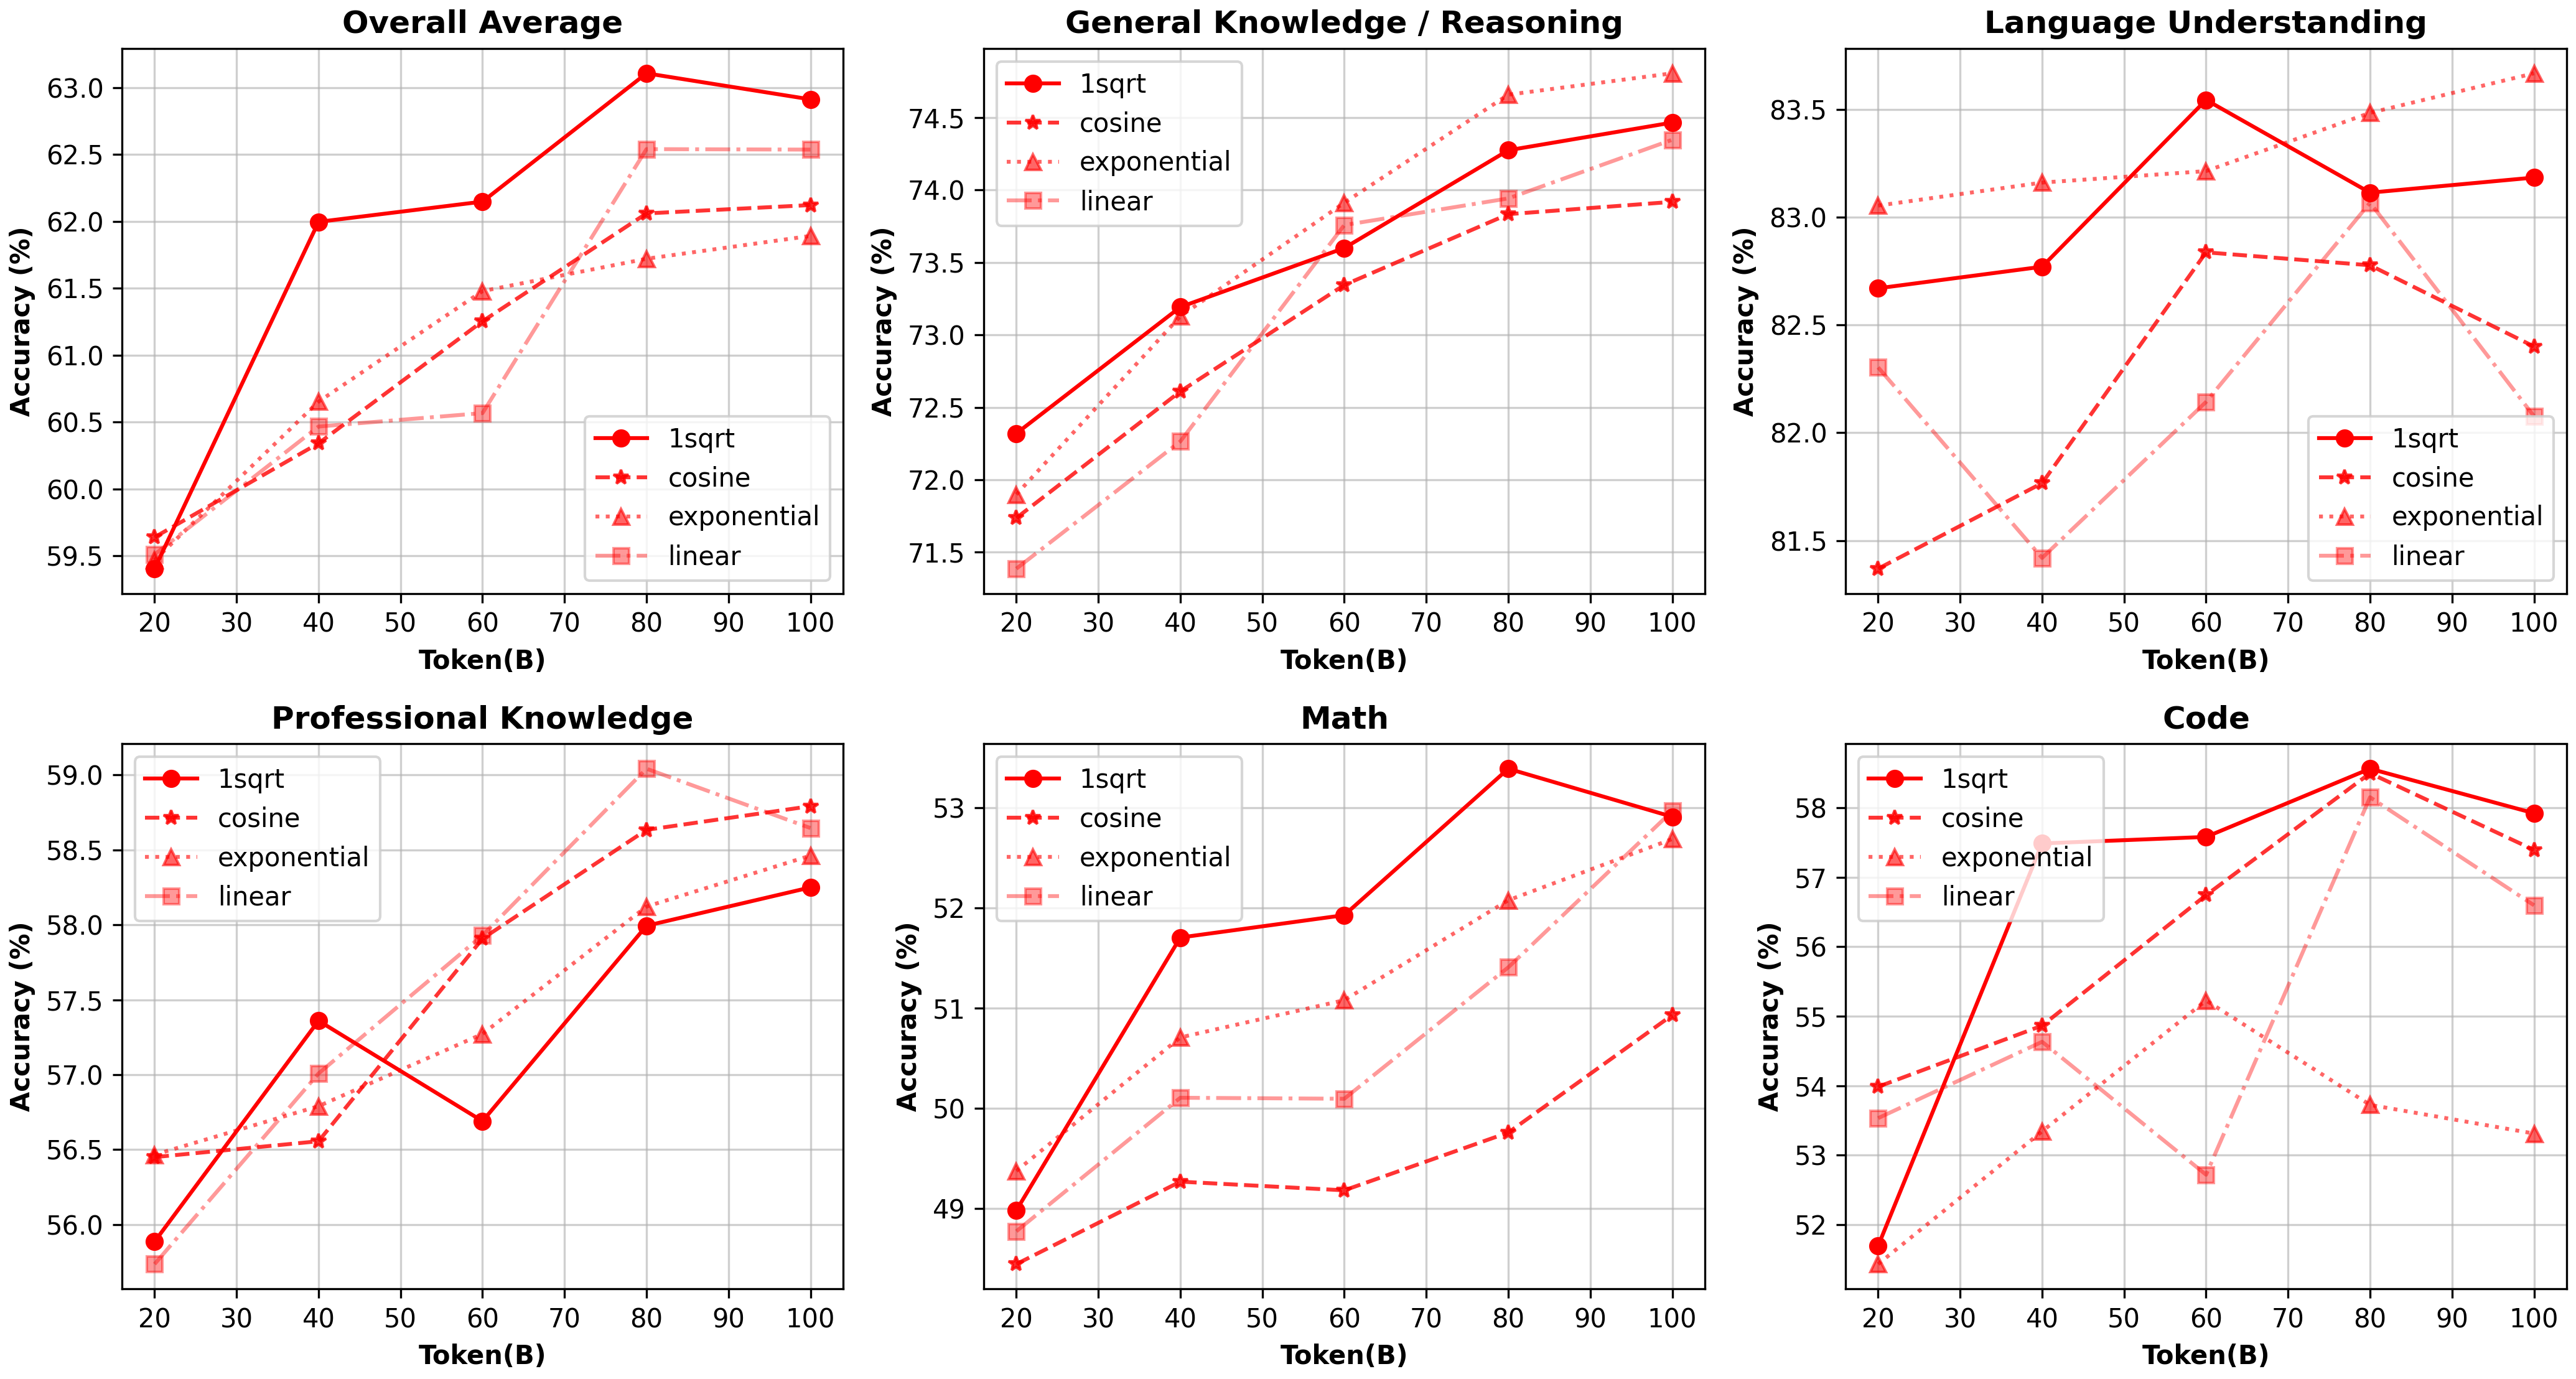
\includegraphics[width=\textwidth]{figs/app_decay.png}
    \caption{\textbf{Comprehensive performance comparison between different decay strategy of WSM schedule.}}
    \label{fig:app_decay}
\end{figure*}







\section{How Checkpoint Merging Influences Network Behavior: Stability \& Generalizability}
\label{parameter}
The architecture composed of sequentially connected transformer blocks has been widely adopted in mainstream LLMs. In such chain-like structures, variations in shallow-layer outputs typically propagate layer-wise. More stable and generalizable input-output patterns exhibit greater potential for enhancing downstream task performance. To investigate how checkpoint merging influences network behavior, we conduct the following analyses:

\paragraph{Stability}
In numerical analysis, the condition number quantifies a function’s sensitivity to input perturbations and the resultant output errors. Remarkably, our analysis in Figure \ref{fig:wss_ling_mini_merge_ckpt_condition_number} reveals that the decay process induces sharp deterioration of condition numbers, whereas checkpoint merging demonstrates superior stability. This indicates that the checkpoint merging strategy not only improves performance but also preserves parametric stability.

\paragraph{Generalizability}
When maintaining competitive performance, higher SVD entropy (singular values entropy) correlates with greater matrix effective rank, indicating greater information capacity in matrix operations. For continue pre-training and fine-tuning scenarios, higher SVD Entropy often means higher potential for model plasticity~\citep{alter2000singular,roy2007effective,liu2025muonscalablellmtraining}. Figure \ref{fig:wss_ling_mini_merge_ckpt_svd_entropy} shows the trend of SVD Entropy during training. We observe that decay is a rapid entropy reduction process, which continuously damages the potential for future continue training of the model. In contrast, the merged models still maintain a higher generalizability, manifested as a higher SVD Entropy.
\begin{figure*}[t]
    \centering
    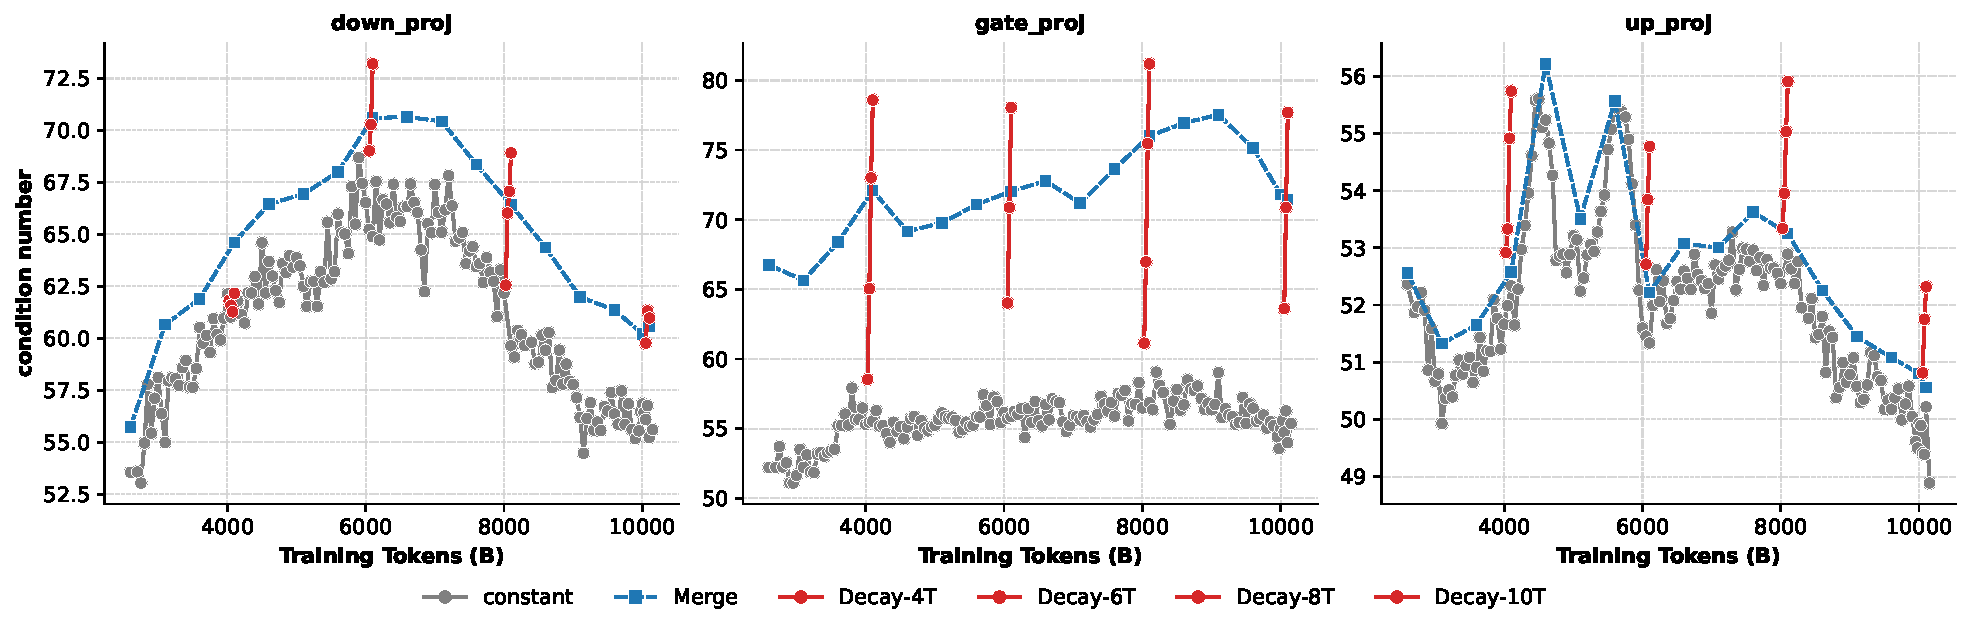
\includegraphics[width=\textwidth]{figs/wss_ling_mini_merge_ckpt_condition_number.pdf}
    \caption{\textbf{Condition number of weight matrices across different training tokens.}}
    \label{fig:wss_ling_mini_merge_ckpt_condition_number}
\end{figure*}

\begin{figure*}[t]
    \centering
    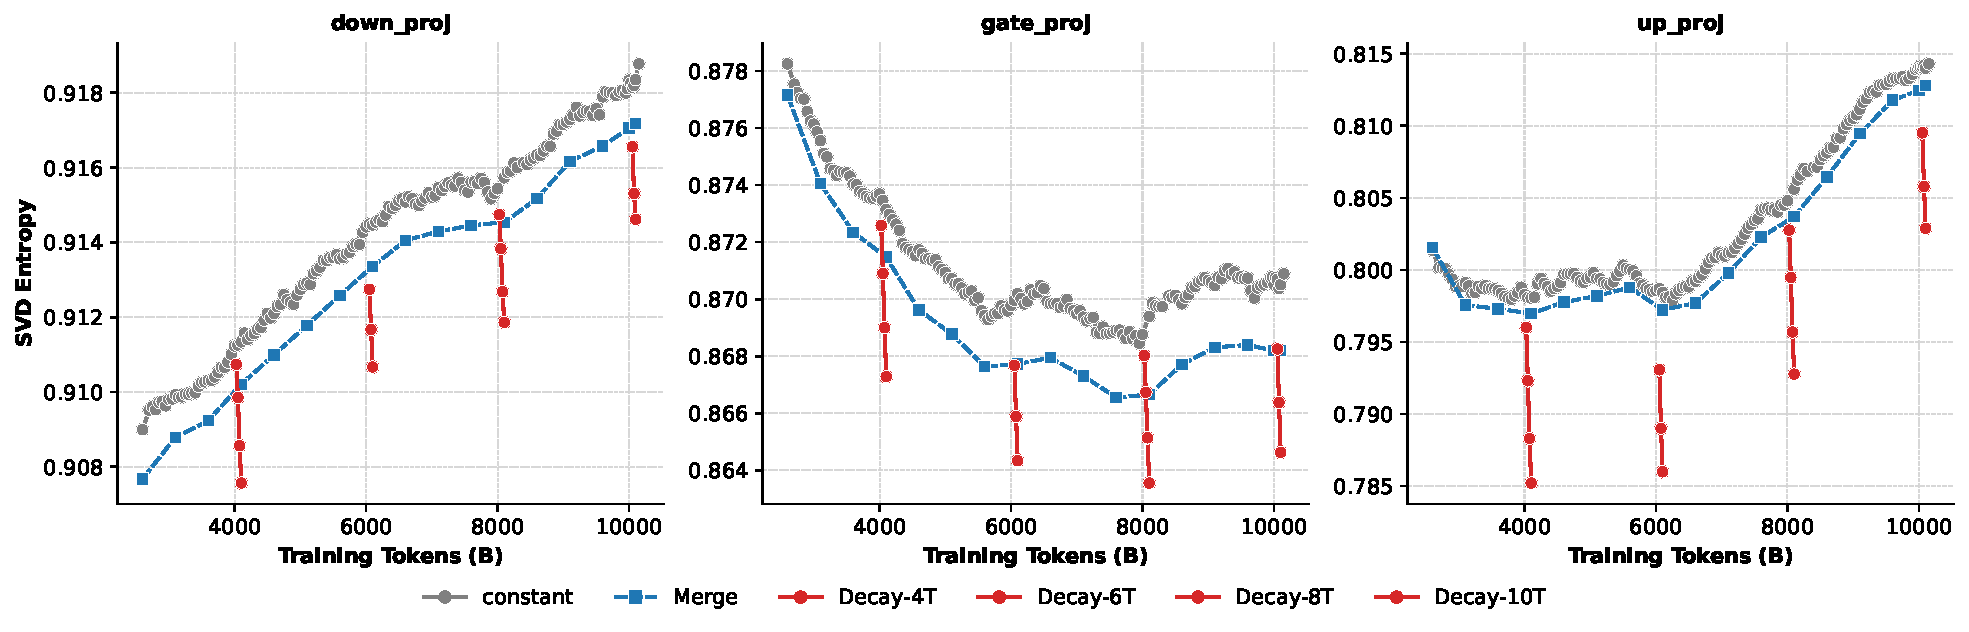
\includegraphics[width=\textwidth]{figs/wss_ling_mini_merge_ckpt_svd_entropy.pdf}
    \caption{\textbf{The entropy of singular values for each weight matrix in the feed-forward network (FFN) layers.}}
    \label{fig:wss_ling_mini_merge_ckpt_svd_entropy}
\end{figure*}








\section{Detailed Evaluation Results}
We provide detailed evaluation results to compare our methods with WSD. Figure \ref{fig:all_datasets} shows a detailed comparison on each dataset across the various categories from the main experiments in Section \ref{sec:main}, where WSM achieves an advantage on the vast majority of datasets. We select the checkpoint with the highest average score for each method, including WSD and the three WSM merging algorithms, and list them in Table \ref{table:sample-table}. Table \ref{inst_dataset_1} and \ref{inst_dataset_2} shows the performance comparison of checkpoints generated by the WSM and WSD schedules after supervised fine-tuning (SFT).
\label{all_datasets}
\begin{figure*}[ht]
    \centering
    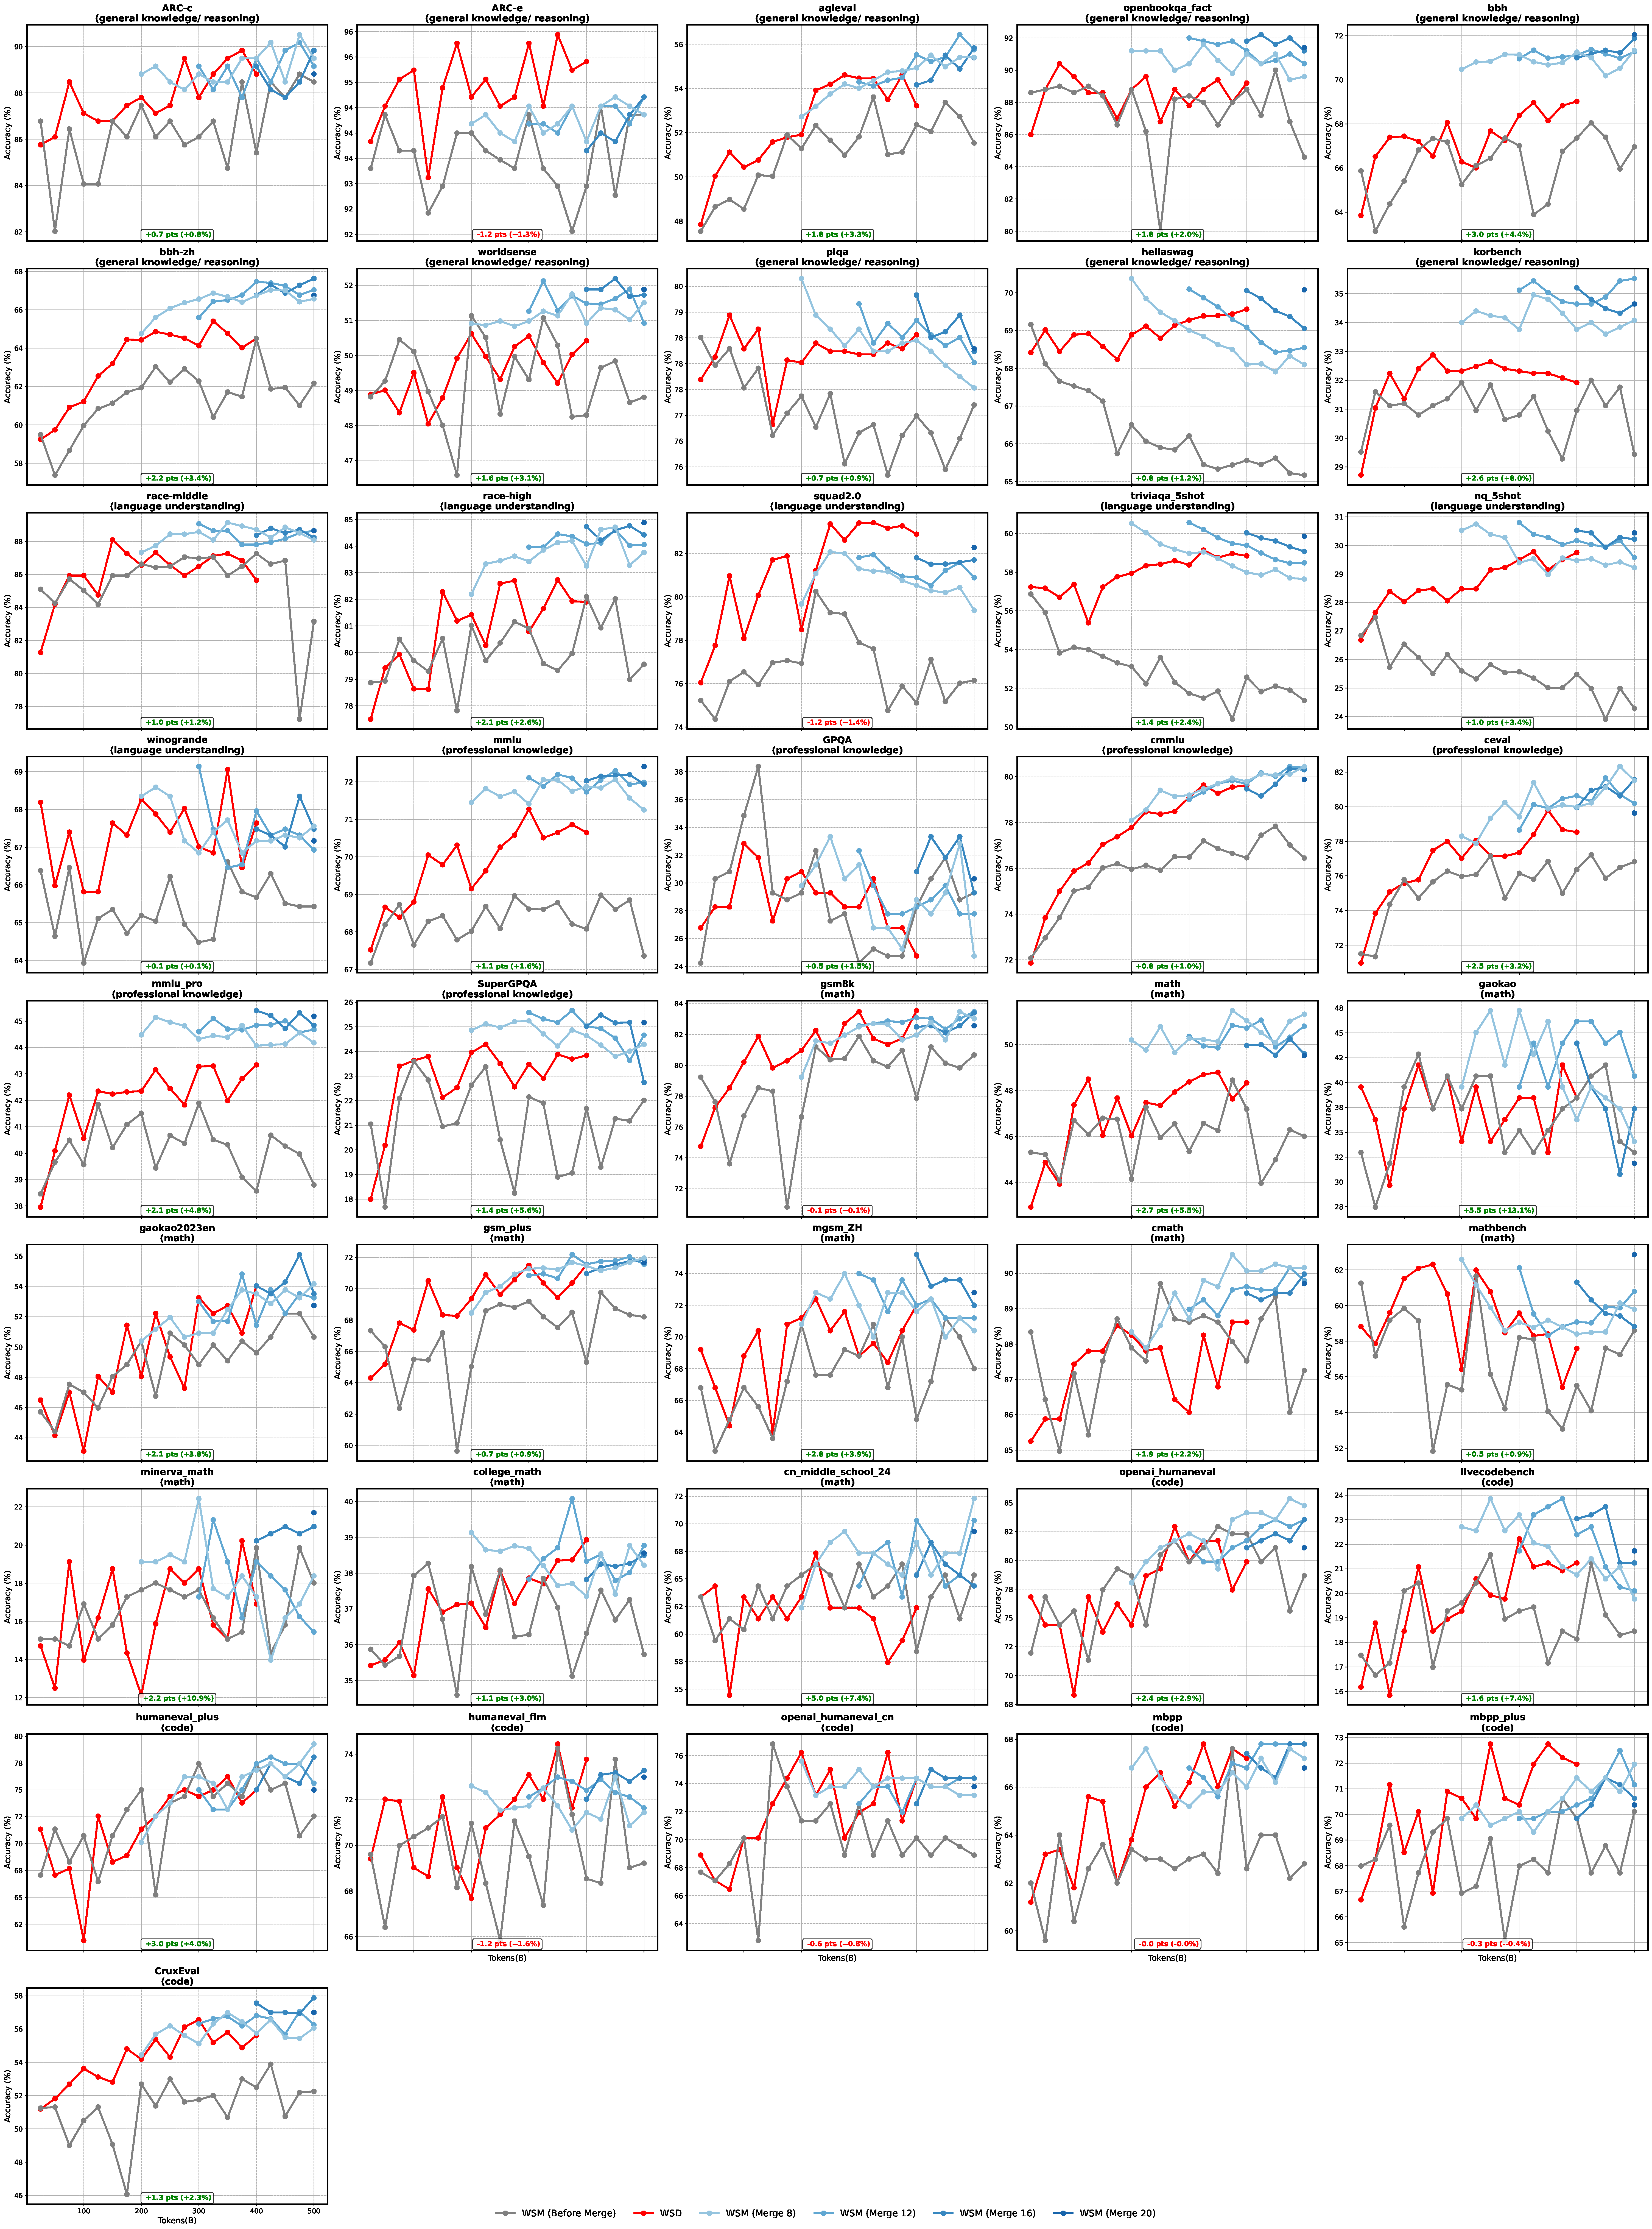
\includegraphics[width=0.95\textwidth]{figs/all_datasets_with_absolute_improvement.pdf}
    \caption{Detailed performance comparison between the standard WSD schedule (via learning rate decay) and our WSM schedule (via checkpoint merging) under different merging durations.}
    \label{fig:all_datasets}
\end{figure*}


\begin{table}[h]
\small
  \caption{\textbf{Detailed performance comparison of base models trained using WSM (with three distinct merging algorithms) versus WSD scheduling approaches.}}
  \label{table:sample-table}
  \centering
  \setlength{\tabcolsep}{5pt} %
  \begin{tabular}{clllllll}
\toprule
\multicolumn{1}{l}{}                           & \multicolumn{1}{l}{\multirow{2}{*}{\textbf{Metric}}} & & \multicolumn{1}{c}{\multirow{2}{*}{\textbf{WSD}}} &  & \multicolumn{3}{c}{\textbf{WSM}} \\ \cmidrule(l){5-8} 
\multicolumn{1}{l}{}                           & \multicolumn{1}{c}{} & \multicolumn{1}{c}{}               &      &  & \textbf{EMA}    & \textbf{mean}  & \textbf{1-\textit{sqrt}}  \\
\midrule
\multirow{10}{*}{\shortstack{General Knowledge \\ \& Reasoning}} & ARC-c                  &  & 88.8                                     &  & 87.8   & 88.1  & 89.8   \\
                                               & ARC-e                  &  & 95.4                                     &  & 93.7   & 94.0  & 94.5   \\
                                               & AGIEval                &  & 53.2                                     &  & 53.8   & 54.4  & 54.2   \\
                                               & OpenBookQA\_fact       &  & 89.2                                     &  & 89.2   & 92.2  & 91.8   \\
                                               & BBH                    &  & 69.0                                     &  & 70.0   & 71.2  & 71.0   \\
                                               & BBH-zh                 &  & 64.5                                     &  & 65.3   & 67.3  & 66.5   \\
                                               & WorldSense             &  & 50.4                                     &  & 50.6   & 51.9  & 52.1   \\
                                               & PIQA                   &  & 78.6                                     &  & 78.2   & 78.5  & 78.5   \\
                                               & HellaSwag              &  & 69.6                                     &  & 68.2   & 69.9  & 69.7   \\
                                               & KOR-Bench               &  & 31.9                                     &  & 33.7   & 34.8  & 34.6   \\
\midrule
\multirow{8}{*}{\shortstack{Language \\ Understanding}}        & race-middle            &  & 85.7                                     &  & 88.7   & 88.8  & 87.9   \\
                                               & race-high              &  & 81.9                                     &  & 82.2   & 84.2  & 83.9   \\
                                               & SQuAD2.0               &  & 82.9                                     &  & 81.6   & 81.5  & 81.3   \\
                                               & TriviaQA\_5shot        &  & 58.8                                     &  & 57.5   & 59.8  & 59.7   \\
                                               & NQ\_5shot              &  & 29.8                                     &  & 29.1   & 30.4  & 30.3   \\
                                               & WinoGrande             &  & 67.6                                     &  & 66.7   & 67.3  & 66.6   \\
\midrule
\multirow{6}{*}{\shortstack{Professional \\ Knowledge}}        & MMLU                   &  & 70.7                                     &  & 71.2   & 72.2  & 72.1   \\
                                               & GPQA                   &  & 24.8                                     &  & 30.8   & 33.3  & 30.8   \\
                                               & CMMLU                  &  & 79.6                                     &  & 78.3   & 79.2  & 79.3   \\
                                               & MMLU-Pro              &  & 43.3                                     &  & 43.8   & 45.2  & 44.7   \\
                                               & SuperGPQA              &  & 23.8                                     &  & 24.3   & 25.5  & 25.7   \\
                                               & C-Eval                  &  & 78.5                                     &  & 78.3   & 80.9  & 79.9   \\
\midrule
\multirow{11}{*}{\shortstack{Math}}                         & gsm8k                  &  & 83.6                                     &  & 82.0   & 82.6  & 82.3   \\
                                               & MATH                   &  & 48.3                                     &  & 50.8   & 50.0  & 49.6   \\
                                               & gaokao                 &  & 38.5                                     &  & 47.3   & 39.6  & 48.4   \\
                                               & gaokao2023en           &  & 54.0                                     &  & 49.1   & 53.5  & 53.0   \\
                                               & gsm\_plus              &  & 71.5                                     &  & 69.3   & 71.4  & 70.9   \\
                                               & mgsm\_zh               &  & 72.0                                     &  & 73.2   & 73.2  & 72.8   \\
                                               & CMATH                  &  & 88.6                                     &  & 88.4   & 89.3  & 89.2   \\
                                               & MathBench              &  & 57.6                                     &  & 61.8   & 60.3  & 61.6   \\
                                               & minerva\_math          &  & 16.9                                     &  & 19.9   & 20.6  & 19.1   \\
                                               & college\_math          &  & 38.9                                     &  & 37.8   & 38.3  & 39.0   \\
                                               & cn\_middle\_school\_24 &  & 62.4                                     &  & 67.3   & 68.3  & 70.3   \\
\midrule
\multirow{8}{*}{\shortstack{Code}}                          & HumanEval      &  & 79.9                                     &  & 80.5   & 81.7  & 81.1   \\
                                               & LiveCodeBench          &  & 21.2                                     &  & 20.3   & 23.2  & 22.7   \\
                                               & HumanEval\_plus        &  & 75.0                                     &  & 75.6   & 77.4  & 77.4   \\
                                               & HumanEval\_fim         &  & 73.8                                     &  & 69.3   & 73.1  & 73.9   \\
                                               & HumanEval\_cn  &  & 74.4                                     &  & 77.4   & 75.0  & 75.6   \\
                                               & MBPP                   &  & 67.2                                     &  & 65.0   & 66.8  & 66.8   \\
                                               & MBPP\_plus             &  & 72.0                                     &  & 70.6   & 70.4  & 70.6   \\
                                               & CruxEval               &  & 55.6                                     &  & 54.8   & 57.0  & 57.4  \\
\bottomrule
\end{tabular}
\end{table}




\begin{table}[h]
\small
  \caption{Detailed performance comparison of checkpoints generated by the WSM and WSD schedule after supervised fine-tuning (SFT). Both base checkpoints are fine-tuned under identical settings for 5 epochs. Results are reported based on the epoch with the highest average benchmark score.}
  \label{inst_dataset_1}
  \centering
  \setlength{\tabcolsep}{5pt} %
\begin{tabular}{ccccll}
\toprule
\textbf{}                            & \textbf{}                                                                                       & \textbf{Metric}            &  & \textbf{WSD}   & \textbf{WSM}   \\ \midrule

\multirow{14}{*}{{Knowledge}} & \multirow{6}{*}{{\begin{tabular}[c]{@{}c@{}}Basic\\      Knowledge\end{tabular}}}        & ARC-c               &  & 90.85 & 89.49 \\
                                     &                                                                                                 & BoolQ               &  & 84.80  & 85.38 \\
                                     &                                                                                                 & GaokaoBench         &  & 75.70  & 79.95 \\
                                     &                                                                                                 & AGIEval             &  & 61.87 & 65.22 \\
                                     &                                                                                                 & NQ                  &  & 25.4  & 26.43 \\
                                     &                                                                                                 & TriviaQA            &  & 53.93 & 55.52 \\ \cmidrule{2-6} 
                                     & {Average}                                                                                &                     &  & 65.42 & 67.00    \\ \cmidrule{2-6} 
                                     & \multirow{6}{*}{{\begin{tabular}[c]{@{}c@{}}Professional\\      Knowledge\end{tabular}}} & C-Eval               &  & 76.37 & 77.87 \\
                                     &                                                                                                 & CMMLU               &  & 76.13 & 76.78 \\
                                     &                                                                                                 & MMLU                &  & 72.76 & 74.59 \\
                                     &                                                                                                 & MMLU-Pro           &  & 46.09 & 49.67 \\
                                     &                                                                                                 & GPQA                &  & 29.55 & 33.4  \\
                                     &                                                                                                 & SuperGQPA           &  & 26.50  & 26.43 \\ \cmidrule{2-6} 
                                     & {Average}                                                                                &                     &  & 54.57 & 56.46 \\ \midrule
\multirow{18}{*}{{Code}}      & \multirow{6}{*}{{Code Completion}}                                                       & HumanEval           &  & 85.90  & 86.20  \\
                                     &                                                                                                 & HumanEval\_plus     &  & 81.10  & 80.95 \\
                                     &                                                                                                 & HumanEval\_cn       &  & 78.20  & 76.07 \\
                                     &                                                                                                 & CruxEval            &  & 59.69 & 58.88 \\
                                     &                                                                                                 & Multiple            &  & 66.14 & 64.75 \\
                                     &                                                                                                 & HumanEvalFix        &  & 63.01 & 62.50  \\ \cmidrule{2-6} 
                                     & {Average}                                                                                &                     &  & 72.34 & 71.56 \\ \cmidrule{2-6} 
                                     & \multirow{6}{*}{{Code Generation}}                                                      & MBPP                &  & 81.03 & 81.97 \\ 
                                     &                                                                                                 & MBPP\_plus          &  & 73.02 & 71.43 \\
                                     &                                                                                                 & LiveCodeBench       &  & 31.31 & 33.31 \\
                                     &                                                                                                 & BigCodeBench        &  & 33.77 & 33.16 \\
                                     &                                                                                                 & CodeForces          &  & 19.60  & 18.07 \\
                                     &                                                                                                 & Bird-SQL            &  & 25.95 & 28.10  \\ \cmidrule{2-6} 
                                     & {Average}                                                                                &                     &  & 44.11 & 44.34  \\ \midrule
\multirow{18}{*}{{Math}}      & \multirow{5}{*}{{Elementary Mathematics}}                                                & CMATH               &  & 93.08 & 93.99 \\
                                     &                                                                                                 & gsm8k               &  & 87.34 & 87.79 \\
                                     &                                                                                                 & cn\_middle\_school\_24 &  & 72.28 & 73.27 \\
                                     &                                                                                                 & mgsm\_zh            &  & 76.80  & 78.25 \\
                                     &                                                                                                 & gsm\_plus           &  & 77.28 & 77.93 \\ \cmidrule{2-6} 
                                     & {Average}                                                                                &                     &  & 81.36 & 82.25 \\ \cmidrule{2-6} 
                                     & \multirow{7}{*}{{Intermediate Mathematics}}                                              & MATH                &  & 74.24 & 77.08 \\
                                     &                                                                                                 & MathBench           &  & 74.72 & 75.74 \\
                                     &                                                                                                 & college math        &  & 43.57 & 43.52 \\
                                     &                                                                                                 & gaokao              &  & 64.17 & 60.77 \\
                                     &                                                                                                 & minerva math        &  & 55.74 & 57.31 \\
                                     &                                                                                                 & gaokao2023en        &  & 63.12 & 65.19 \\
                                     &                                                                                                 & MATH500             &  & 74.75 & 77.05 \\ \cmidrule{2-6} 
                                     & {Average}                                                                                &                     &  & 64.33 & 65.24 \\ \cmidrule{2-6} 
                                     & \multirow{3}{*}{{Advanced Mathematics}}                                                  & OlympiadBench       &  & 41.89 & 41.93 \\
                                     &                                                                                                 & AIME2024            &  & 11.04 & 11.67 \\
                                     &                                                                                                 & AIME2025            &  & 11.46 & 12.71 \\ \cmidrule{2-6} 
                                     & {Average}                                                                                &                     &  & 21.46 & 22.10  \\ 
\bottomrule
\end{tabular}
\end{table}


\begin{table}[h]
\small
  \caption{\textbf{Detailed performance comparison of checkpoints generated by the WSM and WSD schedule after supervised fine-tuning (SFT).} Both base checkpoints are fine-tuned under identical settings for 5 epochs. Results are reported based on the epoch with the highest average benchmark score.}
  \label{inst_dataset_2}
  \centering
  \setlength{\tabcolsep}{5pt} %
\begin{tabular}{ccccll}
\toprule
\textbf{}                            & \textbf{}                                                                                       & \textbf{Metric}            &  & \textbf{WSD}   & \textbf{WSM}   \\ \midrule
\multirow{5}{*}{{Language}}   & \multirow{4}{*}{{Language Understanding}}                                                & C3                  &  & 84.38 & 87.18 \\
                                     &                                                                                                 & WSC                 &  &  69.23     & 77.88 \\
                                     &                                                                                                 & race-high           &  & 82.93 & 84.65 \\
                                     &                                                                                                 & race-middle         &  & 87.95 & 89.42 \\ \cmidrule{2-6} 
                                     & {Average}                                                                                &                     &  & 81.12 & 84.78 \\ \midrule
\multirow{11}{*}{{Reasoning}} & \multirow{10}{*}{{Complex Reasoning}}                                                    & bbh                 &  & 72.87 & 73.97 \\
                                     &                                                                                                 & drop                &  & 76.41 & 78.66 \\
                                     &                                                                                                 & hellaswag           &  & 68.11 & 70.93 \\
                                     &                                                                                                 & ocnli               &  & 51.32 & 52.75 \\
                                     &                                                                                                 & piqa                &  & 81.50  & 82.92 \\
                                     &                                                                                                 & ProntoQA            &  & 37.00    & 38.00    \\
                                     &                                                                                                 & Multi-LogiEval      &  & 0.27  & 56.68 \\
                                     &                                                                                                 & MuSR                &  & 48.53 & 51.33 \\
                                     &                                                                                                 & korbench            &  & 37.52 & 37.52 \\
                                     &                                                                                                 & bbh-zh              &  & 69.38 & 71.47 \\ \cmidrule{2-6} 
                                     & {Average}                                                                                &                     &  & 63.21 & 64.94 \\ \midrule
\multirow{9}{*}{{Agent}}      & \multirow{5}{*}{{Tool-use}}                                                              & teval\_v2\_en       &  & 84.4  & 86.16 \\
                                     &                                                                                                 & teval\_v2\_zh       &  & 83.49 & 84.72 \\
                                     &                                                                                                 & BFCL\_AST           &  & 79.35 & 78.30  \\
                                     &                                                                                                 & BFCL-Live           &  & 68.33 & 71.39 \\
                                     &                                                                                                 & NEXUS               &  & 30.51 & 29.21 \\ \cmidrule{2-6} 
                                     & {Average}                                                                                &                     &  & 69.22 & 69.96 \\ \cmidrule{2-6} 
                                     & \multirow{2}{*}{{Instruction Following}}                                                 & IFEval              &  & 71.9  & 75.71 \\ 
                                     &                                                                                                 & alignbench          &  & 59.10  & 59.80  \\ \cmidrule{2-6} 
                                     & {Average}                                                                                &                     &  & 65.5  & 67.75 \\ 
\bottomrule
\end{tabular}
\end{table}



